\documentclass[11pt,twoside=semi,openright,numbers=noenddot]{article}

\def\ncode {LPHYS1303}
\def\ncourse {Projet différences finies}
\def\nlecturer {M. Crucifix}
\def\nyear {2021}
\def\ntitle {Mécanique Céleste}

\usepackage{amsmath}
\usepackage{amssymb}
\usepackage{amsthm}
\usepackage[T1]{fontenc}
\usepackage[french]{babel} % traduction
\usepackage[usenames,svgnames,dvipsnames]{xcolor}
\usepackage[hang, small, labelfont=bf, up, textfont=it]{caption} % custom caption under figures
%\usepackage{bookmark}
%\usepackage{booktabs} % beautiful tables
%\usepackage[thicklines]{cancel} % cancel terms in equation
%\usepackage{color} % colors in box (theorems,...)
%\usepackage{enumerate}
\usepackage{float}
\usepackage{framed} % box around text
\usepackage{fancyhdr} % header
%\usepackage{fancyvrb}
\usepackage{mathrsfs}
\usepackage{mathtools}
\usepackage[parfill]{parskip} % avoid bad alignment in paragraphs
\usepackage{pgfplots} % plot in tikz
\usepackage{braket} % braket and sets
\usepackage{derivative} % derivatives
\usepackage{siunitx}
\usepackage{silence} % silence useless warnings
\usepackage{tikz}
\usepackage{tkz-euclide}
\usepackage{tikz-3dplot}
\usepackage{units} % Non-stacked fractions and better unit spacing
\usepackage{xspace} % prints a trailing space in a smart way.

\usetikzlibrary{calc,patterns,angles,quotes}

\tikzset{circ/.style = {fill, circle, inner sep = 0, minimum size = 3}}
\tikzset{scirc/.style = {fill, circle, inner sep = 0, minimum size = 1.5}}
\tikzset{mstate/.style={circle, draw, blue, text=black, minimum width=0.7cm}}

% \titlespacing*{\section}{0pt}{5.5ex plus 1ex minus .2ex}{4.3ex plus .2ex}
% \titlespacing*{\subsection}{0pt}{5.5ex plus 1ex minus .2ex}{4.3ex plus .2ex}

\usepackage{enumitem}
\setlist{nosep,after=\vspace{\baselineskip}}

\pgfplotsset{compat=1.12}
\sisetup{locale = FR}

\usepackage[marginparwidth=2cm]{geometry}
\geometry{
	paper=a4paper,
	inner=2.0cm,
	outer=3.0cm,
	bindingoffset=.5cm,
	top=3.5cm,
	bottom=3.5cm
}

\usepackage{graphicx}
\setkeys{Gin}{width=\linewidth,totalheight=\textheight,keepaspectratio}
%\graphicspath{{figures/}}

% Default images settings
\setkeys{Gin}{width=\linewidth, totalheight=\textheight, keepaspectratio}

%---------------------------------------------------
% BUGGY PACKAGES THAT NEED TO BE LOADED AT THE END
%---------------------------------------------------

% colored hyperlink
% load hyperref at the end to avoid conflicts
\usepackage[colorlinks]{hyperref} % colored ref
% % cleverref must be loaded after hyperref
% \usepackage{cleveref} % create ref

\hypersetup{
  colorlinks=true,
  linkcolor=blue,
  filecolor=blue,
  citecolor=black,
  urlcolor=cyan
}

% conditions for equations
% https://tex.stackexchange.com/questions/95838/how-to-write-a-perfect-equation-parameters-description
\newenvironment{conditions}
  {\par\vspace{\abovedisplayskip}\noindent\begin{tabular}{>{$}l<{$} @{${}={}$} l}}
	{\end{tabular}\par\vspace{\belowdisplayskip}}

\newenvironment{conditions*}
  {\par\vspace{\abovedisplayskip}\noindent
   \tabularx{\columnwidth}{>{$}l<{$} @{${}={}$} >{\raggedright\arraybackslash}X}}
  {\endtabularx\par\vspace{\belowdisplayskip}}

%----------------
% FIX
%----------------

\setlength{\headheight}{14.5pt}

% increase vertical space for aligned equations
\setlength{\jot}{7pt}

% Filter warnings issued by package biblatex starting with "Patching footnotes failed"
\WarningFilter{biblatex}{Patching footnotes failed}

%----------------------
%	COMMANDS
%----------------------

% commands shortcuts
\newcommand{\mb}{\mathbb}
\newcommand{\R}{\mb{R}}
\newcommand{\Z}{\mb{Z}}
\newcommand{\N}{\mb{N}}
\newcommand{\C}{\mb{C}}
\newcommand{\A}{\mb{A}} % hypersphere area
\newcommand{\V}{\mb{V}} % hypersphere volume
\newcommand{\dS}{\cdot d\vb{S}}
\newcommand{\lag}{\mathcal{L}}
\newcommand{\ham}{\mathcal{H}}
\newcommand{\Mod}[1]{\ \mathrm{mod}\ #1}

\renewcommand{\vec}[1]{\mathbf{#1}} % bold vectors
\newcommand{\vd}[1]{\dot{\vec{#1}}}
\newcommand{\vdd}[1]{\ddot{\vec{#1}}}

% norm
\newcommand{\bignorm}[1]{\left\lVert#1\right\rVert}

% smaller overline (line above variable)
\newcommand{\overbar}[1]{\mkern 1.5mu\overline{\mkern-1.5mu#1\mkern-1.5mu}\mkern 1.5mu}

% prints an asterisk that takes up no horizontal space.
% useful in tabular environments.
\newcommand{\hangstar}{\makebox[0pt][l]{*}}

% Prints argument within hanging parentheses (i.e., parentheses that take
% up no horizontal space). Useful in tabular environments.
\newcommand{\hangp}[1]{\makebox[0pt][r]{(}#1\makebox[0pt][l]{)}}

% cancel terms with color
% \newcommand{\ccancel}[2]{\renewcommand{\CancelColor}{\color{#2}}\bcancel{#1}}

% small parallel
\makeatletter
\newcommand{\newparallel}{\mathrel{\mathpalette\new@parallel\relax}}
\newcommand{\new@parallel}[2]{%
  \begingroup
  \sbox\z@{$#1T$}% get the height of an uppercase letter
  \resizebox{!}{\ht\z@}{\raisebox{\depth}{$\m@th#1/\mkern-5mu/$}}%
  \endgroup
}
\makeatother

\renewcommand*\contentsname{Table des matières}


\begin{document}

\showthe\textwidth
\showthe\columnwidth

\begin{titlepage}
  \newcommand{\HRule}{\rule{\linewidth}{0.1mm}} 
  \center % Center everything on the page
   
  %-------------------------------------------------------------------------
  %	HEADING SECTIONS
  %-------------------------------------------------------------------------
  \textsc{\Large \ncode}\\[0.5cm] % course code
  \textsc{\Large \ncourse}\\[0.5cm] % course name
  \textsc{\large \nlecturer}\\[0.5cm] % course lecturer
  
  %-------------------------------------------------------------------------
  %	TITLE SECTION
  %-------------------------------------------------------------------------
  
  \HRule \\[0.4cm]
  { \huge \bfseries  \ntitle}\\[0.1cm]
  \HRule \\[1.5cm]
  
  %\includegraphics{uclouvain.jpg} % \\[0.5cm] % 
  \vfill
\end{titlepage}

\fancyhead[R]{\thepage}
\fancyhead[L]{\rightmark}
\cfoot{}
\pagestyle{fancy}

\tableofcontents
\newpage

Le but de ce projet est de simuler l'évolution de l'orbite de Jupiter pour les $5000$ prochaines années. Dans un premier temps nous ne tiendrons compte que de Jupiter et du Soleil (\textbf{problème à 2 corps}) et nous ajouterons par la suite la contribution de Saturne (\textbf{problème à 3 corps}).

Afin d'illustrer ces évolutions orbitales, nous mettrons en oeuvre 3 schémas numériques différents à savoir les schémas de \emph{Heun}, \emph{Euler symplectique} et \emph{Stormer-Verlet}. Nous verrons que ce premier ne conserve pas l'énergie tandis que ces 2 derniers sont symplectiques c'est à dire qu'ils conservent la structure Hamiltonienne du système.

\section{Dérivation des équations canoniques}
\subsection{Problème à 2 corps}

Soit $m_1$ la masse du Soleil et $m_2$ la masse de Jupiter avec $m_1 \gg m_2$ et soit $\vec{r}_1$ la position du Soleil et $\vec{r}_2$ la position de Jupiter avec $\vec{r} = |\vec{r}_1 - \vec{r}_2|$ leur distance relative.

Prenons la coordonnée généralisée $\vec{q} = \vec{r} \in \R^3$.

L'énergie cinétique du système est,
\begin{align*}
  T &= \sum_{i=1}^{2} T_i \\
    &= \frac{1}{2} m_1 \vd{r}_1^2 + \frac{1}{2} m_2 \vd{r}_2^2
\end{align*}

L'énergie potentielle est,
\begin{equation*}
  V = V(|\vec{r}_1 - \vec{r}_2|) = - \frac{Gm_1m_2}{|\vec{r}_1 - \vec{r}_2|}
\end{equation*}
avec $G$ la constante universelle de gravitation.

Le Lagrangien est donc,
\begin{equation}
  \lag = \frac{1}{2} m_1 \vd{r}_1^2 + \frac{1}{2} m_2 \vd{r}_2^2 + \frac{Gm_1m_2}{|\vec{r}_1 - \vec{r}_2|}
\end{equation}

Lorsqu'on cherche une solution analytique, il est judicieux de réexprimer le Lagrangien en terme du mouvement relatif $\vec{r}$ et du mouvement du centre de masse $\vec{r}_{CM}$ et de passer en coordonnées sphériques. Ce n'est pas d'utilité dans le cas de notre résolution numérique.

L'Hamiltonien est la transformée de legendre du Lagrangien et est donc donné par,
\begin{align}
  \ham
    &= \sum_{i=1}^2 \vec{p}_i \cdot \vec{r}_i - \lag \\
    &= \frac{\vec{p}_1^2}{2m_1} + \frac{\vec{p}_2^2}{2m_2} - \frac{Gm_1m_2}{|\vec{r}_1 - \vec{r}_2|}
\end{align}
 où $\vec{p}_i$ est l'impulsion conjuguée de la i-ème masse.

Les équations canoniques d'un hamiltonien $\mathcal{H}$ quelconque sont données par,
\begin{equation} \label{eq:canonical-equations}
 \dot{p}_i = -\pdv{\ham}{r_i} \quad ; \quad \dot{r_i} = \pdv{\ham}{p_i}
\end{equation}
pour $i = \set{x,y,z}$ et $(r_x, r_y, r_z) = (x, y, z)$.

\subsection{Problème à 3 corps et généralisation à N corps}
Dans notre simulation, nous voulons également prendre en compte la présence de \textbf{Saturne}. Plutôt que de dériver chaque fois les équations canoniques lorsque l'on introduit un nouveau corps, nous allons généraliser au cas d'un problème à $N$ corps.

Nous prenons en compte tous les potentiels d'interaction entre les différentes masses. L'Hamiltonien devient,
\begin{equation}
    \ham = \sum_{i=1}^N \frac{\vec{p}_i^2}{2m_i} + \sum_{1\leq i<j \leq N} \frac{Gm_i m_j}{|\vec{r}_i - \vec{r}_j|}
\end{equation}
où $|\vec{r}_i - \vec{r}_j| \equiv \vec{r}_{ij}$ est la distance relative entre la masse $m_i$ et la masse $m_j$.

En utilisant (\ref{eq:canonical-equations}), les équations canoniques pour la i-ème masse sont alors données par,
\begin{align}
  \vd{r}_i =
  \begin{pmatrix}
    \dot{x}_i \\ \dot{y}_i \\ \dot{z}_i
  \end{pmatrix}
  =
  \begin{pmatrix}
    \frac{p_{x_i}}{m_i} \\[6pt]
    \frac{p_{y_i}}{m_i} \\[6pt]
    \frac{p_{z_i}}{m_i}
  \end{pmatrix}
\end{align}
\begin{align}
  \vd{p}_i =
  \begin{pmatrix}
    \dot{p}_{x_i} \\ \dot{p}_{y_i} \\ \dot{p}_{z_i}
  \end{pmatrix}
  =
  \begin{pmatrix}
    \sum_{j \neq i}^{N} - \frac{Gm_im_j}{(\vec{r}_{ij})^3} (x_i - x_j) \\[6pt]
    \sum_{j \neq i}^{N} - \frac{Gm_im_j}{(\vec{r}_{ij})^3} (y_i - y_j) \\[6pt]
    \sum_{j \neq i}^{N} - \frac{Gm_im_j}{(\vec{r}_{ij})^3} (z_i - z_j)
  \end{pmatrix}
\end{align}

\section{Schémas numériques}

Afin d'illustrer l'évolution orbital de notre système planétaire restreint, nous allons utiliser 3 schémas numériques différents à savoir \emph{Heun}, \emph{Euler symplectique} et \emph{Stormer-Verlet}. Nous commençons d'abord par les définir explicitement et à calculer leur ordre de convergence. Pour chaque schéma numérique, nous supposons une équation différentielle donnée par,
\begin{equation} \label{eq:edo}
    \vd{y}(t) \equiv f(t, \vec{y}), \quad f: \R^n \rightarrow \R
\end{equation}

On rappelle par ailleurs que le développement de Taylor à l'ordre $2$ d'une fonction $f: \R^n \rightarrow \R$ autour du point $\vec{a} \in \R^n$ est donné par,
\begin{equation}
    T^2_a f(x) = f(\vec{a}) + Jf(\vec{a})(\vec{x} - \vec{a}) + \frac{1}{2} (\vec{x} - \vec{a})^T Hf(\vec{a})(\vec{x} - \vec{a})
\end{equation}
où $Jf(\vec{a})$ est la matrice Jacobienne de $f$ au point $\vec{a}$ et $Hf(a)$ est la matrice Hessienne de $f$ au point $\vec{a}$.

\subsection{Heun (RK2)}
Soit le schéma de Heun,
\begin{align*}
  \begin{cases}
    \tilde{y}_{j+1} &= y_j + (\Delta t) f(t_j, y_j) \\
    y_{j+1} &= y_j + \frac{1}{2}(k_1 + k_2)
  \end{cases}
\end{align*}

où les coefficients $k_1$ et $k_2$ sont donnés par,
\begin{align*}
  k_1 &= (\Delta t) f(t_j, y_j) \\
  k_2 &= (\Delta t) f (t_{j+1}, \tilde{y}_{j+1})
\end{align*}

Montrons que ce schéma converge à l'ordre $2$ en $\Delta t$. Afin de simplifier les notations, nous noterons $f(t_j, y_j) \equiv f_j$

Nous avons,
\begin{align}
  y_{j+1}
    &= y_{j} + \frac{1}{2}(\Delta t) f_j + \frac{1}{2}(\Delta t) f(t_{j+1}, \tilde{y}_{j+1})
\end{align}

Nous effectuons un développement de Taylor à l'ordre 2 de $f(t_{j+1}, \tilde{y}_{j+1})$ autour du point $\vec{a} = (t_j, y_j)$,
\begin{align}
  f(t_{j+1}, \tilde{y}_{j+1})
    &= f_j + \pdv{f_j}{t}(t_{j+1} - t_j) + \pdv{f_j}{y}(\tilde{y}_{j+1} - y_j) + \frac{1}{2} \pdv[2]{f_j}{t}(t_{j+1} - t_j)^2 \\
    &+ \frac{1}{2} \pdv[2]{f_j}{y}(\tilde{y}_{j+1} - y_j) + \frac{1}{2} \pdv{f_j}{t,y}(t_{j+1} - t_j)(\tilde{y}_{j+1} - y_j) \\
    &= f_j + \pdv{f_j}{t}(\Delta t) + \pdv{f_j}{y}(\Delta t f_j) + \frac{1}{2} \pdv[2]{f_j}{t}(\Delta t)^2 \\
    &+ \frac{1}{2} \pdv[2]{f_j}{y}([\Delta t]^2[f_j]^2) + \frac{1}{2} \pdv{f_j}{t,y}([\Delta t]^2 f_j)
\end{align}

Ce qui nous donne pour le schéma de Heun,
\begin{align}
    y_{j+1} = y_j + (\Delta t)f_j + \frac{(\Delta t)^2}{2} \left( \pdv{f_j}{t} + \pdv{f_j}{y}f_j \right) + \frac{(\Delta t)^3}{4} \left( \pdv[2]{f_j}{t} + \pdv[2]{f_j}{y}(f_j^2) + \pdv{f_j}{t,y}(f_j) \right)
\end{align}

On regarde au schéma de Taylor à l'ordre 2,
\begin{align}
  y_{j+1}
    &= y_j + (\Delta t) y^{(1)}(t_j) + \frac{1}{2!}(\Delta t)^2 y^{(2)}(t_j)
\end{align}
Or nous savons que
\begin{equation}
  y^{(2)}(t_j) = \odv*{\dot{y}(t_j)}{t} = \odv*{[f(t_j, y_j)]}{t} = \left(\pdv{f_j}{t} + \pdv{f_j}{y}\dot{y} \right) = \left(\pdv{f_j}{t} + \pdv{f_j}{y}f_j \right)
\end{equation}

Donc,
\begin{equation}
  y_{j+1} = y_j + (\Delta t) f_j + \frac{(\Delta t)^2}{2} \left(\pdv{f_j}{t} + \pdv{f_j}{y}f_j \right)
\end{equation}

On effectue la différence du Heun avec le schéma de Taylor et on observe que,
\begin{equation}
  y_{\text{Heun}} - y_{\text{Taylor}} = \mathcal{O}((\Delta t)^3)
\end{equation}

Par conséquent, l'erreur commise à chaque pas de temps est de l'ordre de $(\Delta t)^3$ et puisque cette différence tend vers zéro pour $(\Delta t) \rightarrow 0$, on trouve que la méthode de Heun est convergente à l'ordre $\tau = ((\Delta t)^2)$.

\subsection{Euler symplectique}
Soit le schéma d'Euler symplectique,
\begin{align*}
    p_{j+1}
        &= p_j - (\Delta t) \pdv{\ham(q_j, p_j)}{q} \\
    q_{j+1}
        &= q_j + (\Delta t) \pdv{\ham(q_j, p_{j+1})}{p}
\end{align*}

Montrons que ce schéma converge à l'ordre $1$. Afin de simplifier les notations, nous noterons $f_j \equiv \pdv{\ham}{q}(q_j, p_j)$ et $g_j \equiv \pdv{\ham}{p}(q_j, p_j)$.

Nous avons,
\begin{equation}
  q_{j+1} = q_j + (\Delta t) g(q_j, p_{j+1})
\end{equation}

Effectuons un développement de Taylor à l'orde $2$ de $g(q_j, p_{j+1})$ autour du point $\vec{a} = (q_j, p_j)$.
\begin{align}
    g(q_j, p_{j+1})
        &= g_j + \pdv{g_j}{q}(q_{j+1} - q_j) + \pdv{g_j}{p}(p_{j+1} - p_j) \\
        &+ \frac{1}{2}\pdv[2]{g_j}{q}(q_{j+1} - q_j)^2 + \frac{1}{2}\pdv[2]{g_j}{p}(p_{j+1} - p_j)^2 \\
        &+ \frac{1}{2}\pdv{g_j}{q,p}(q_{j+1} - q_j)(p_{j+1} - p_j) \\
        &= g_j + \pdv{g_j}{q}((\Delta t)g_j)- \pdv{g_j}{p}((\Delta t) f_j) \\
        &+ \frac{1}{2}\pdv[2]{g_j}{q}((\Delta t)g_j)^2 - \frac{1}{2}\pdv[2]{g_j}{p}((\Delta t) f_j)^2 + \frac{1}{2}\pdv{g_j}{q,p}((\Delta t)g_j)((\Delta t) f_j)
\end{align}

Ce qui nous donne pour le schéma d'Euler symplectique à l'ordre $2$,
\begin{align}
    q_{j+1}
      &= q_j + (\Delta t) g_j  + (\Delta t)^2 \left( \pdv{g_j}{q}(g_j) - \pdv{g_j}{p}(f_j) \right) \\
      &+ \frac{(\Delta t)^3}{2} \left(\pdv[2]{g_j}{q}(g_j)^2  - \pdv[2]{g_j}{p}(f_j)^2 +\pdv{g_j}{q,p}(g_j f_j) \right)
\end{align}

On regarde au schéma de Taylor à l'ordre $2$,
\begin{align}
  q_{j+1}
    &= q_j + (\Delta t) q^{(1)}(t_j) + \frac{1}{2!}(\Delta t)^2 q^{(2)}(t_j)
\end{align}

Nous savons que,
\begin{equation}
  q^{(1)}(t_j) = \pdv{\ham(q_j, p_j)}{p} \equiv g_j
\end{equation}
Et que,
\begin{align}
  q^{(2)}(t_j) = \odv{g_j}{t} = \odv*{[g(q_j, p_j)]}{t} = \pdv{g_j}{q}\dot{q} + \pdv{g_j}{p}\dot{p} = \pdv{g_j}{q}g_j - \pdv{g_j}{p}f_j
\end{align}

Donc,
\begin{equation}
  q_{j+1} = q_j + (\Delta t) g_j + \frac{(\Delta t)^2}{2} \left( \pdv{g_j}{q}g_j - \pdv{g_j}{p}f_j \right)
\end{equation}

% TODO: finish taylor shit

On observe que le schéma de Taylor diffère du schéma d'Euler symplectique à partir de l'ordre $2$.
\begin{align*}
    q_{Taylor} - q_{Euler} &= \mathcal{O}((\Delta t)^2)
\end{align*}

Par conséquent, l'erreur commise à chaque pas de temps est de l'ordre de $(\Delta t)^2$ et puisque cette différence tend vers zéro pour $(\Delta t) \rightarrow 0$, on trouve que la méthode d'Euler symplectique est convergente à l'ordre $\tau = \Delta t$.

\subsection{Stormer-Verlet}
Le schéma de Stormer-Verlet est donné par les équations suivantes,
\begin{align*}
    p_{j+\frac{1}{2}} &= p_j - \frac{(\Delta t)}{2} \pdv{\ham}{q}(q_j, p_j) \\
    q_{j+1} &= q_j + (\Delta t) \pdv{\ham}{p}(q_j, p_{j+1/2}) \\
    p_{j+1} &= p_{j+\frac{1}{2}} - \frac{\Delta t}{2} \pdv{\ham}{q}(q_{j+1},  p_{j+1/2})
\end{align*}

Montrons que ce schéma converge à l'ordre 2. Pour simplifier les notations posons $f_j \equiv \pdv{\ham}{q}(q_j, p_j)$ et $g_j \equiv \pdv{\ham}{p}(q_j, p_j)$.

Nous avons,
\begin{equation}
    p_{j+1} = p_j - \frac{(\Delta t)}{2} f_j - \frac{(\Delta t)}{2} f(q_{j+1}, p_{j+1/2})
\end{equation}

Effectuons un développement de Taylor à l'ordre $2$ de $f(q_{j+1}, p_{j+1/2})$ autour de $\vec{a} = (q_j, p_j)$.
\begin{align}
    f(q_{j+1}, p_{j+1/2})
        &= f_j + \pdv{f_j}{q}(q_{j+1 - q_j}) + \pdv{f_j}{p}(p_{j+1/2} - p_j) + \frac{1}{2}\pdv[2]{f_j}{q}(q_{j+1} - q_j)^2 \\
        &+ \frac{1}{2}\pdv[2]{f_j}{p}f_j(p_{j+1/2} - p_j)^2 + \frac{1}{2} \pdv{f_j}{q,p}(q_{j+1} - q_j)(p_{j+1/2} - p_j) \\
        &= f_j + \pdv{f_j}{q} (\Delta t) g(q_j, p_{j+1/2}) - \pdv{f_j}{p}\frac{(\Delta t)}{2}f_j + \frac{1}{2}\pdv[2]{f_j}{q}((\Delta t)^2 g^2(q_j, p_{j+1/2})) \\
        &+ \frac{1}{2}\pdv[2]{f_j}{p}\left( \frac{(\Delta t)^2}{4} f_j^2 \right) + \frac{1}{2}\pdv{f_j}{q,p}\left( (\Delta t) g(q_j, p_{j+1+2}) \frac{\Delta t}{2}f_j \right)
\end{align}

Nous effectuons également un développement de Taylor à l'ordre $2$ de $g_{q_j, p_{j+1/2}}$ atour de $\vec{a} = (q_j, p_j)$.
\begin{align*}
  g(q_j, p_{j+1/2})
    &= g_j + \pdv{g_j}{p}(p_{j+1/2} - p_j) + \frac{1}{2} \pdv[2]{g_j}{p}(p_{j+1/2} - p_j)^2 \\
    &= g_j - \pdv{g_j}{p} \frac{(\Delta t)}{2} f_j + \frac{1}{2} \pdv[2]{g_j}{p}\frac{(\Delta t)^2}{4}(f_j)^2
\end{align*}

Dès lors,
\begin{align}
  p_{j+1}
    &= p_j - \frac{\Delta t}{2}f_j - \frac{\Delta t}{2}f_j - \pdv{f_j}{q}\frac{(\Delta t)^2}{2} \left( g_j - \pdv{g_j}{p}\frac{\Delta t}{2}f_j + \frac{1}{2}\pdv[2]{g_j}{p} \frac{(\Delta t)^2}{4}(f_j)^2 \right) \\
    &+ \pdv{f_j}{p}\frac{(\Delta t)^2}{2}f_j - \frac{1}{2}\pdv[2]{f_j}{q}\frac{(\Delta t)^3}{2} \left( g_j - \pdv{g_j}{p}f_j + \frac{1}{2}\pdv[2]{g_j}{p} \frac{(\Delta t)^2}{4}(f_j)^2 \right)^2 \\
    &+ \frac{1}{2}\pdv[2]{f_j}{p}\frac{(\Delta t)^3}{4} (f_j)^2 + \frac{1}{2}\pdv[2]{f_j}{q,p} \frac{(\Delta t)^3}{4}f_j \left( g_j - \pdv{g_j}{p}f_j + \frac{1}{2}\pdv[2]{g_j}{p} \frac{(\Delta t)^2}{4}(f_j)^2 \right) \\
    &= p_j - (\Delta t)f_j - \frac{(\Delta t)^2}{2} \left( \pdv{f_j}{q}g_j - \pdv{f_j}{p}f_j \right) + \mathcal{O}((\Delta t)^3)
\end{align}

Regardons au schéma de Taylor à l'ordre $2$.
\begin{align}
  p_{j+1} = p_j + (\Delta t) p^{(1)}(t_j) + \frac{1}{2!}k^2p^{(2)}(t_j)
\end{align}
Nous savons que,
\begin{equation}
  p^{(1)}(t_j) = - \pdv{\ham(q_j, p_j)}{q} \equiv -f_j
\end{equation}
Et d'autre part que,
\begin{align}
  p^{(2)}(t_j) = - \odv*{f_j}{t}
    &= - \left( \pdv{f_j}{q} \dot{q} + \pdv{f_j}{p} \dot{p} \right) \\
    &= - \left( \pdv{f_j}{q} g_j - \pdv{f_j}{p} f_j \right)
\end{align}

Par conséquent,
\begin{equation}
  p_{j+1} = p_j - (\Delta t) f_j - \frac{(\Delta t)^2}{2} \left( \pdv{f_j}{q} g_j - \pdv{f_j}{p} f_j \right)
\end{equation}

On regarde à la différence entre le schéma de Stormer-Verlet et celui de Taylor,
\begin{equation}
  p_{\text{Stormer-Verlet}} - p_{\text{Taylor}} = \mathcal{O}((\Delta t)^3)
\end{equation}

Par conséquent, l’erreur commise à chaque pas de temps est de l’ordre de $(\Delta t)^3$ et puisque cette différence tend vers zéro pour $(\Delta t) \rightarrow 0$, on trouve que la méthode de \emph{Stormer-Verlet} est convergente à l’ordre $\tau = ((\Delta t)^2)$.

\section{Résultats}
\subsection{Illustration orbitale}
Nous commençons par illustrer l'évolution orbitales pour les 3 schémas numériques présentés plus haut.

\begin{figure}[H]
    \centering
    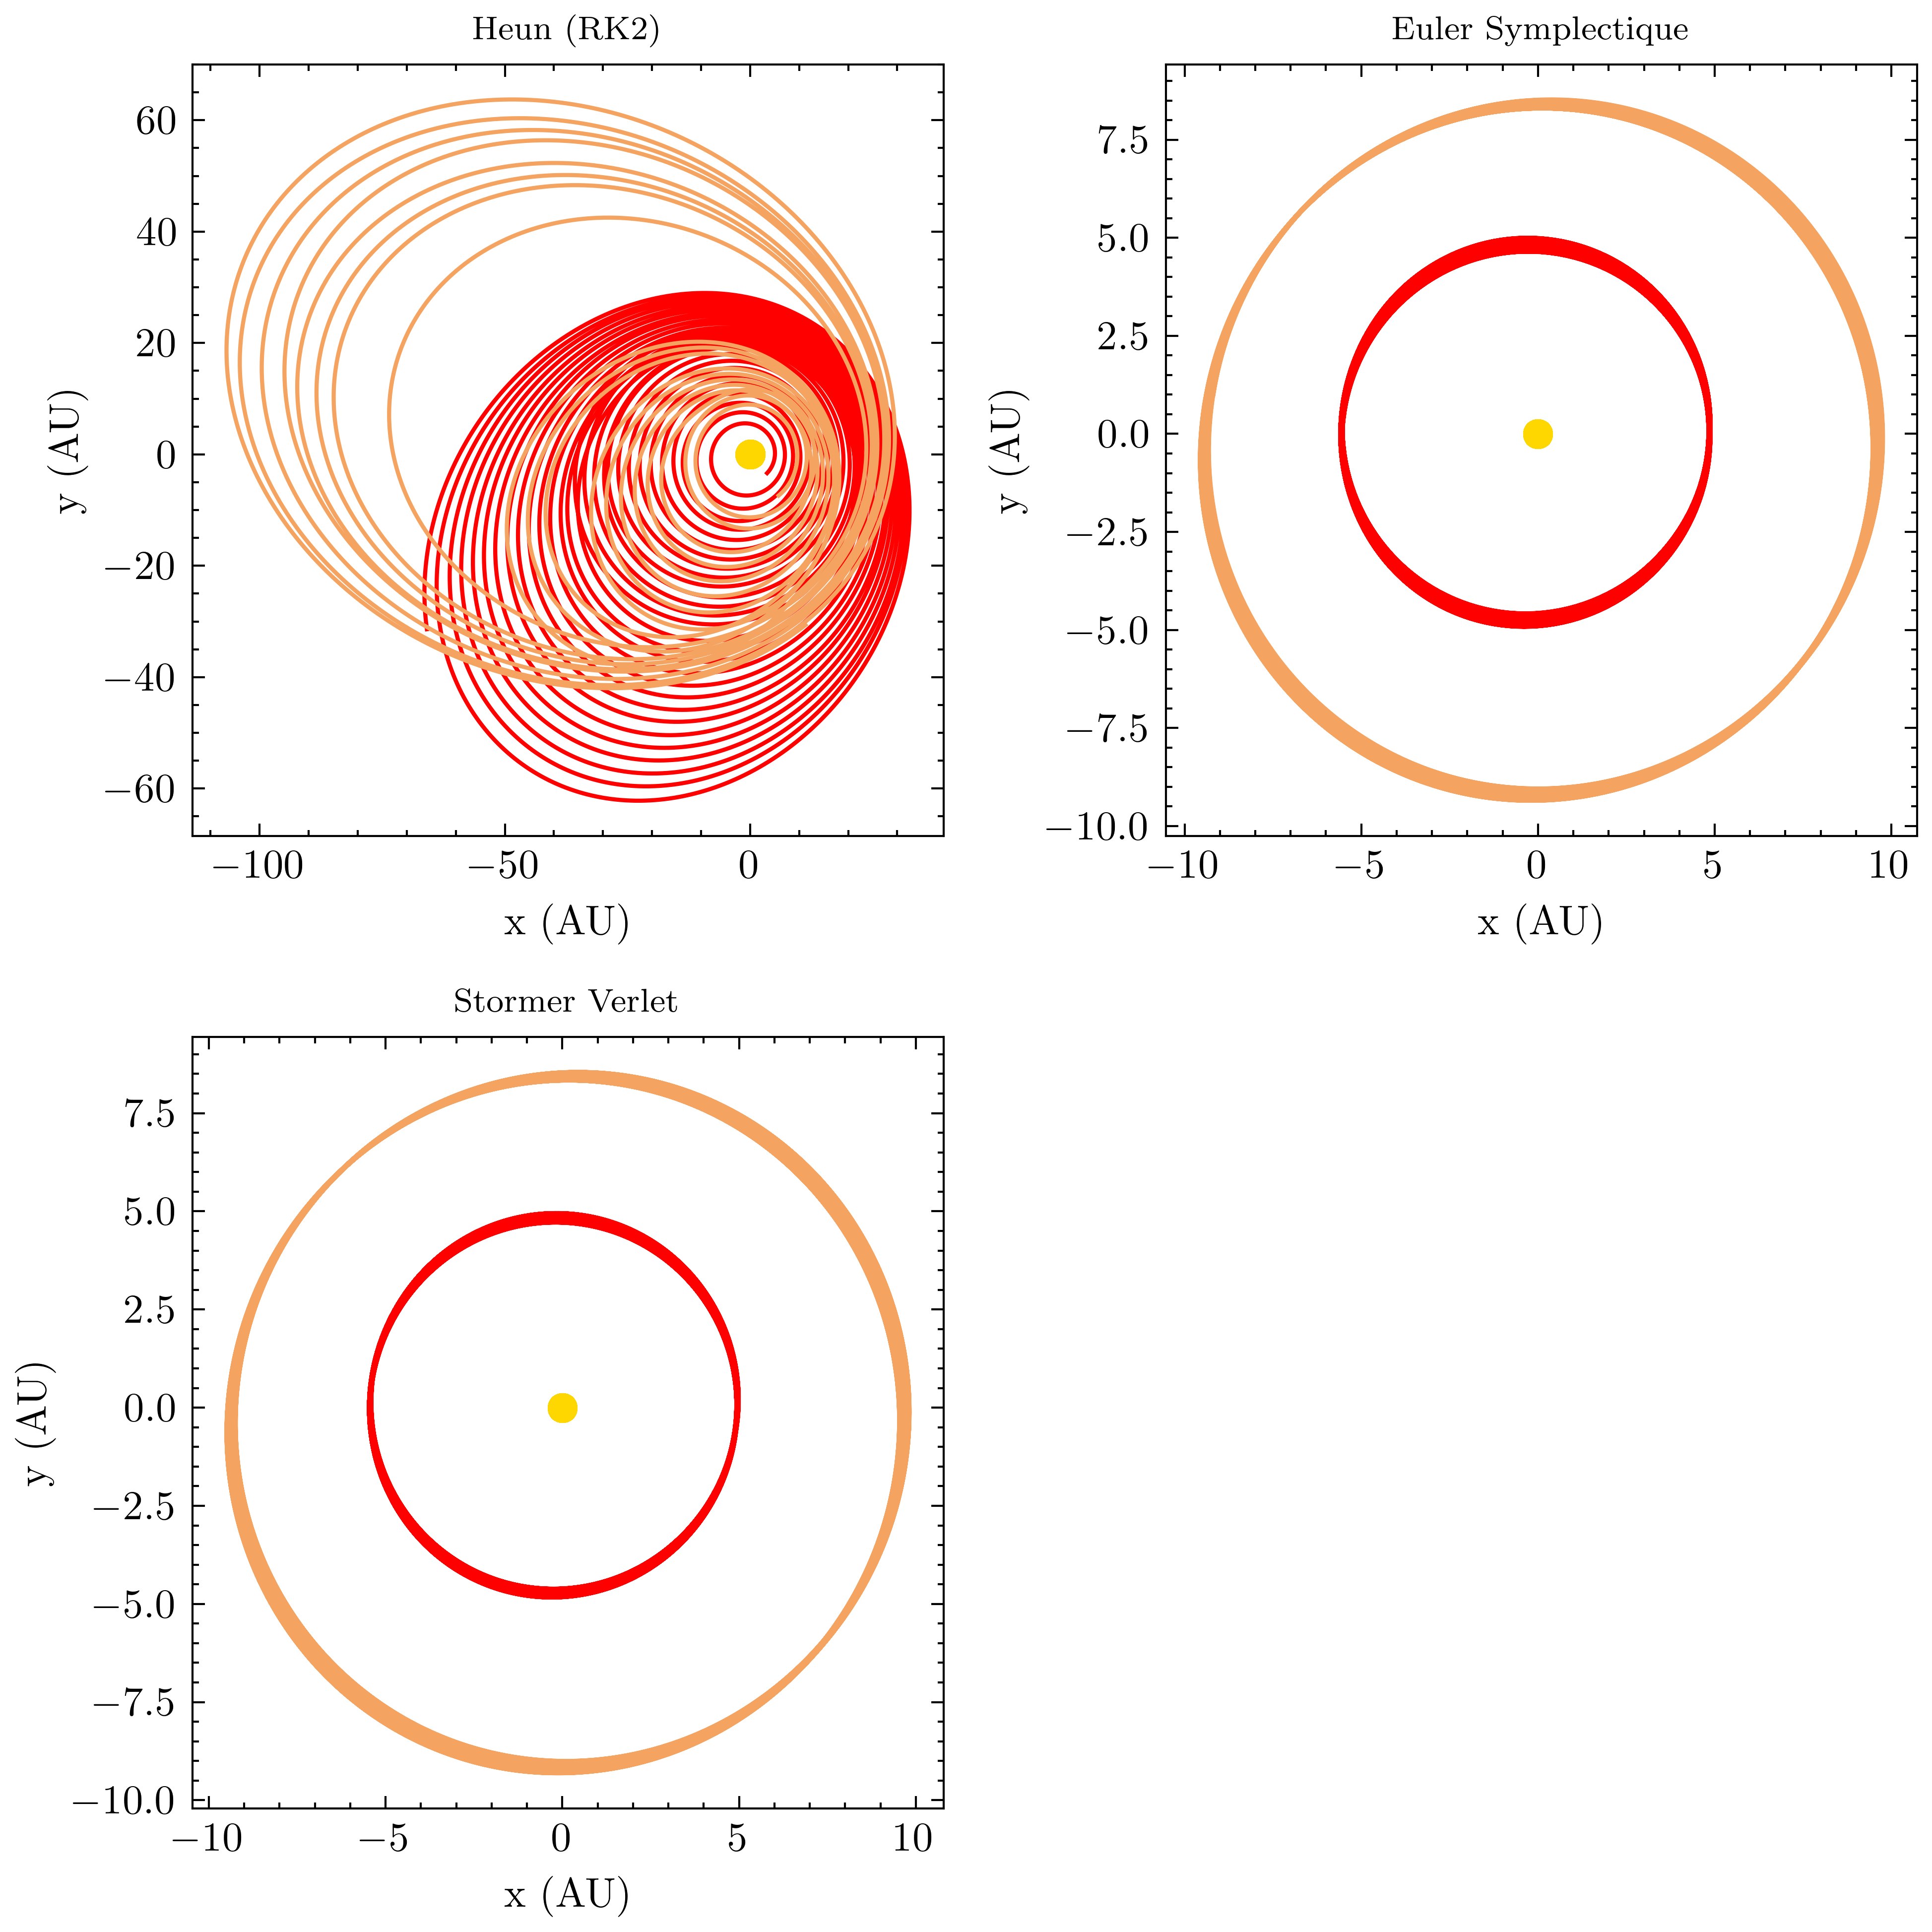
\includegraphics{figures/5000_years/orbital-plot2d.png}
    \caption{Evolution orbitale en 2 dimension de l'orbite du Soleil (\emph{point jaune}), de Jupiter (\emph{rouge}) et de Saturne (\emph{brun}) pour les $5000$ prochaines années.}
    \label{fig:plot2D--5000}
\end{figure}

En en ce qui concerne le schéma de \emph{Heun}, il est clair que les orbites de Saturne et Jupiter dévient fortement de leur trajectoire. Si on réalise une simulation sur $50$ années (\autoref{fig:plot2D--50}), on observe que ces deux planètes dévient fortement de leur trajectoire à chaque révolution autour du Soleil.
Par contre on observe que les orbite de Jupiter et Saturne sont globalement stables pour les 2 schémas symplectiques (\emph{Euler symplectique} et \emph{Stormer-Verlet}). En regardant la \autoref{fig:plot2D--5000}, on remarque en fait que les orbites de Jupiter et Saturne ne sont pas constamment sur la même trajectoire mais qu'il y a de légères fluctuations. Toutefois ces fluctuations sont mineures et la trajectoire de ces orbites est globalement conservée sur $5000$ années. Cela laisse suggérer que l'énergie du système hamiltonien est conservée en moyenne pour les schémas symplectiques. A noter que l'on ne remarque pas ce décalage pour le Soleil étant donné que la position de ce dernier peut-être considérée comme globalement fixe.

\begin{figure}[H]
  \centering
  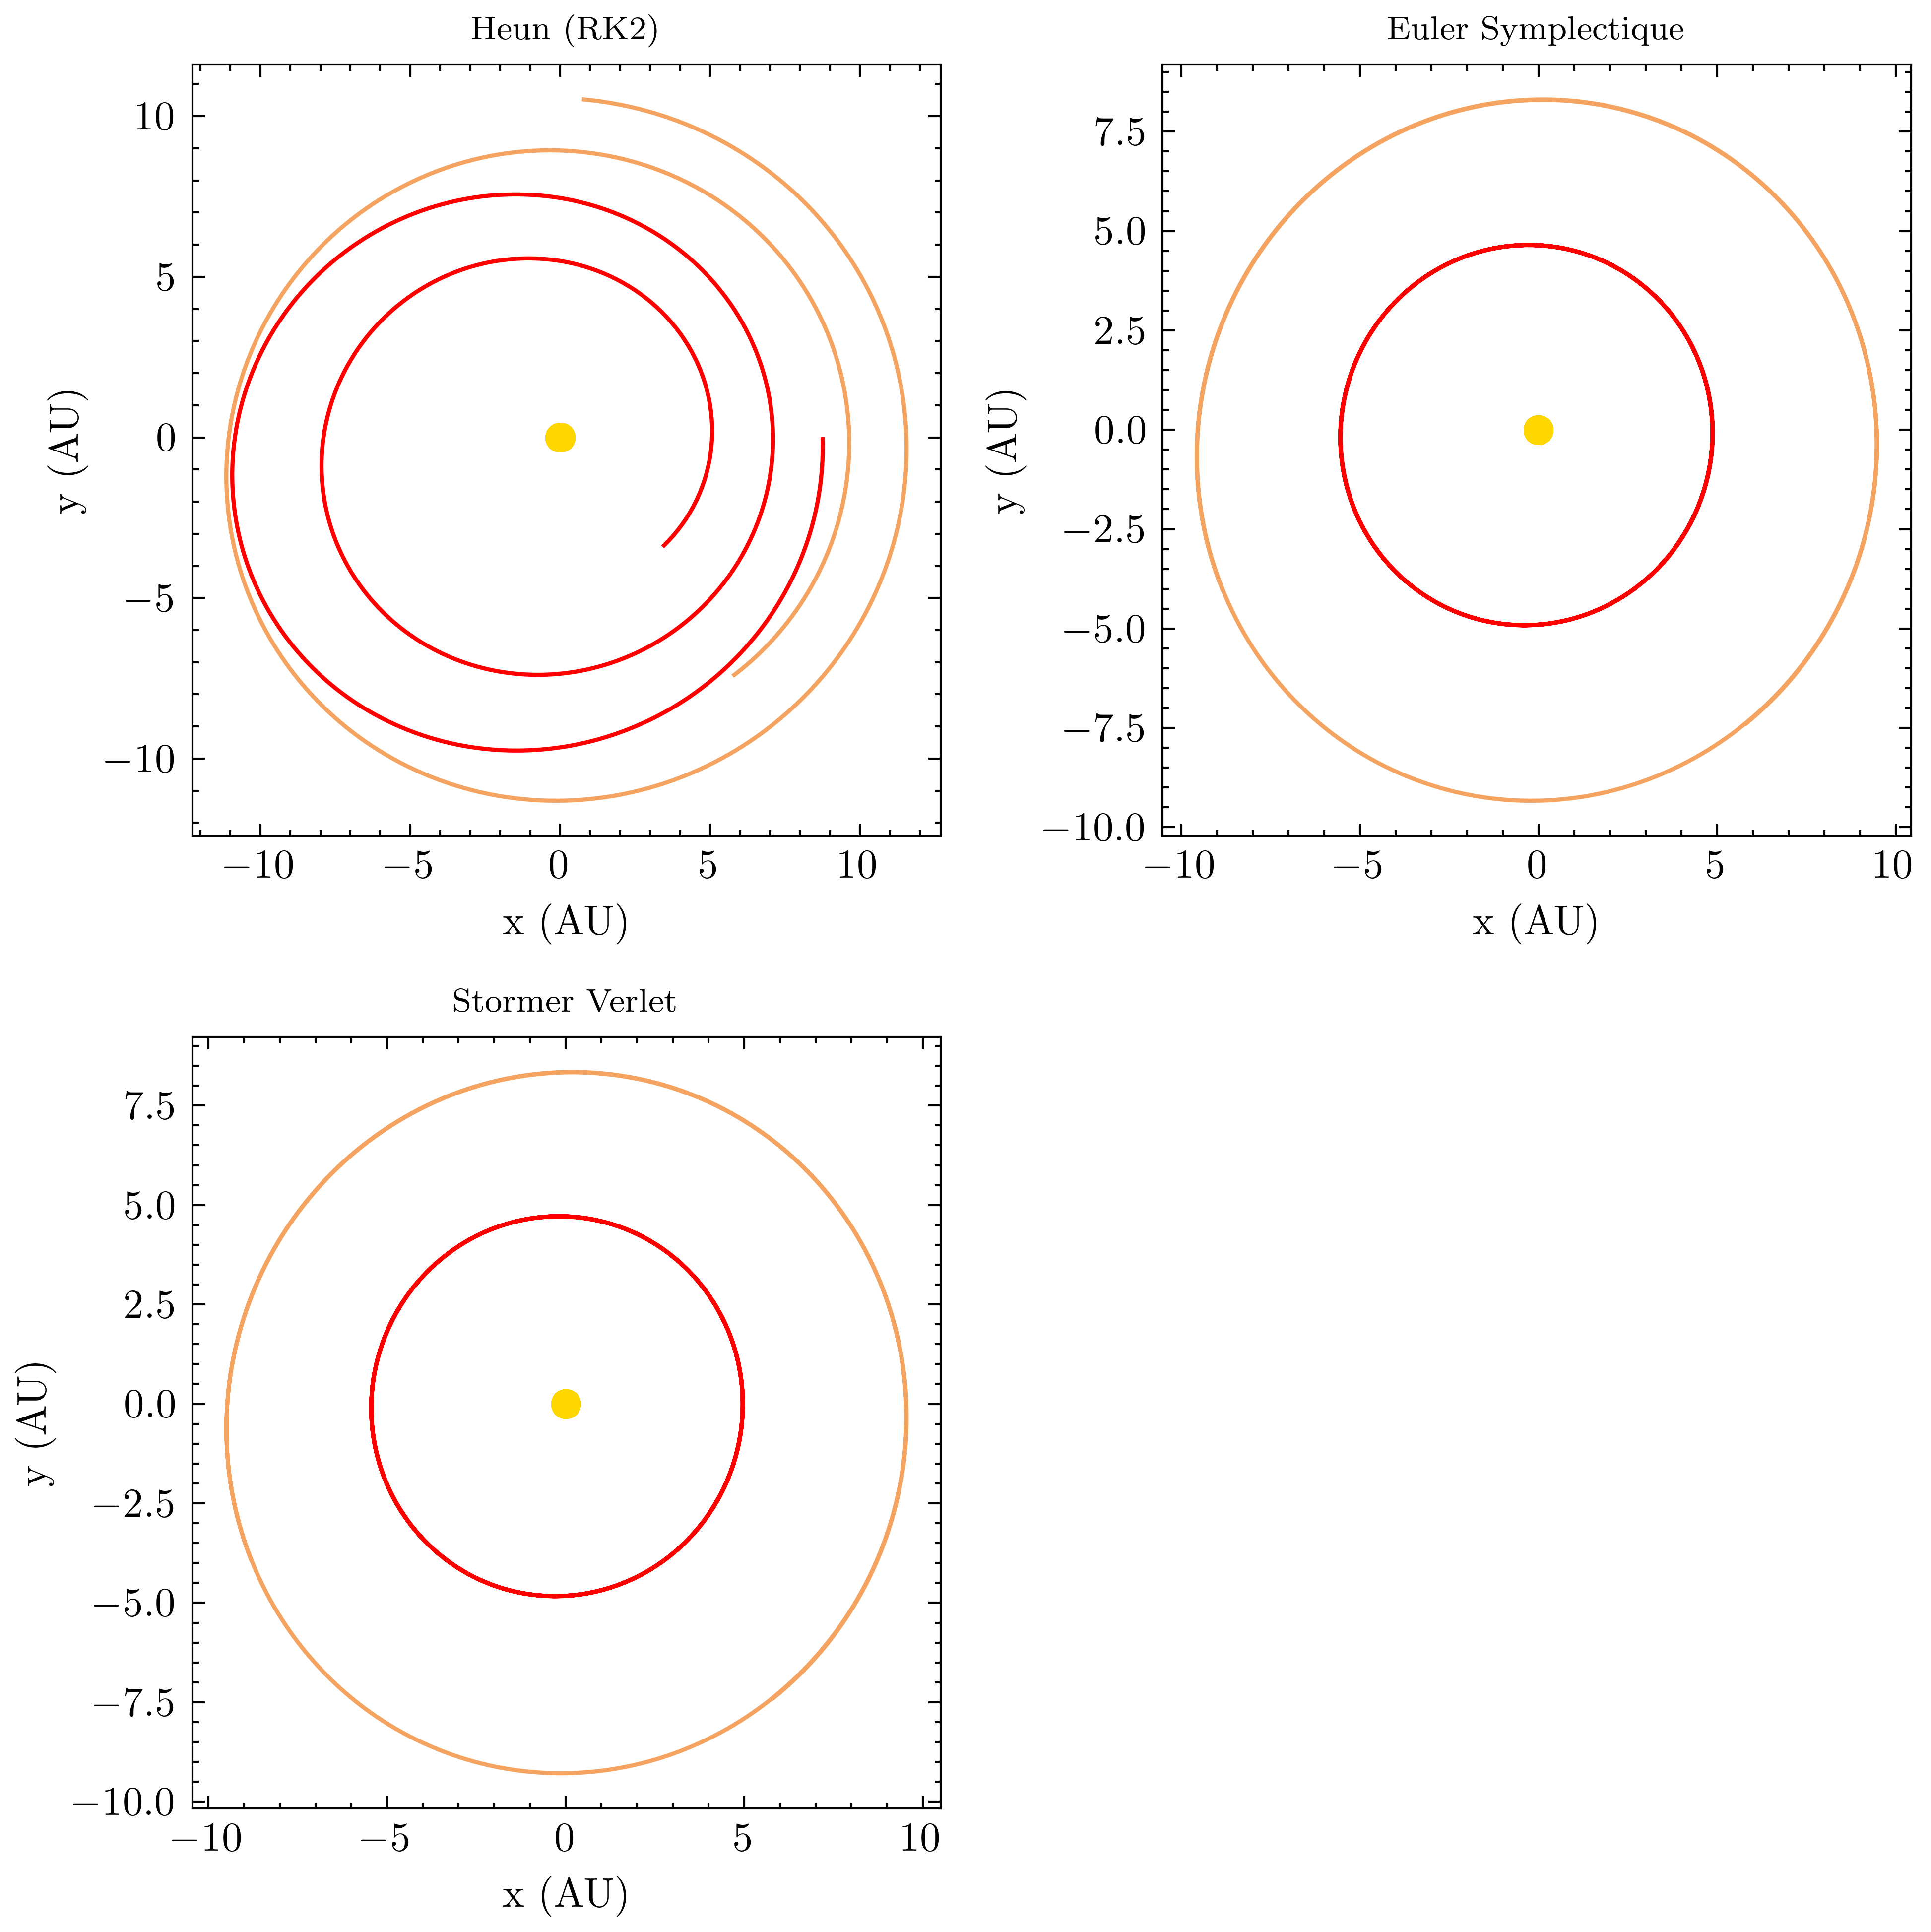
\includegraphics{figures/50_years/orbital-plot2d.png}
  \caption{Evolution orbitale en 2 dimension de l'orbite du Soleil (\emph{point jaune}), de Jupiter (\emph{rouge}) et de Saturne (\emph{brun}) pour les $50$ prochaines années.}
  \label{fig:plot2D--50}
\end{figure}

Nous illustrons maintenant l'évolution d'intégrales premières c'est à dire dans le cas de notre système de quantités conservées telles que l'énergie totale ou encore le moment angulaire. Nous savons qu'en théorie ces 2 quantités sont conservées.

\subsection{Conservation de l'énergie}

L'Hamiltonien du système étant la somme de l'énergie cinétique et potentielle de celui-ci. On peut directement calculer l'énergie du système en fonction du temps en calculant l'Hamiltonien total du système.

\begin{figure}[H]
    \centering
    \includegraphics{figures/5000_years/orbital-energy.pdf}
    \caption{Variation de l'énergie du système du système à 3 corps sur \textbf{$5000$ années} pour les différents schémas numériques utilisés. En \emph{bleu canard} pour le schéma de \textbf{Heun}, en \emph{orange} pour l'\textbf{Euler symplectique} et en \emph{rouge} pour le \textbf{Stormer-Verlet}.}
    \label{fig:orbital-energy--5000}
\end{figure}

Nous voyons que pour le schéma de Heun, il y a une perte d'énergie au cours du temps ce qui explique le décalage dans l'orbite de Saturne et Jupiter pour ce même schéma. Pour les 2 schémas symplectiques, nous observons que l'énergie est variable mais oscille autour d'une certaine valeur d'énergie. C'est à dire que la structure Hamiltonienne du système est conservée (\emph{i.e. le théorème de Liouville est respecté -- LMAT1261}). Cette oscillation est mieux visible si on considère une simulation sur $50$ années

\begin{figure}[H]
  \centering
  \includegraphics{figures/50_years/orbital-energy.pdf}
  \caption{Variation de l'énergie du système à 3 corps sur \textbf{$50$ années} pour les différents schémas numériques utilisés. En \emph{bleu canard} pour le schéma de \textbf{Heun}, en \emph{orange} pour l'\textbf{Euler symplectique} et en \emph{rouge} pour le \textbf{Stormer-Verlet}.}
  \label{fig:orbital-energy--50}
\end{figure}


Etant donné que la période de révolution est grande devant la période de fluctuation de l'énergie, l'orbite est stable pour les 2 schémas symplectiques.

\subsection{Conservation du moment angulaire}
Nous analysons dès à présent la variation du moment angulaire du système $\vec{L} = \sum_{i=1}^{N} \vec{l}_i$ en fonction du temps. Si ce dernier est conservé alors le mouvement orbital est plan.

\begin{figure}[H]
    \centering
    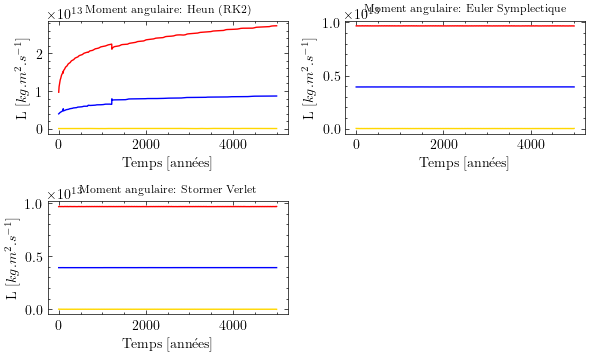
\includegraphics{figures/5000_years/orbital-angular-momentum.pdf}
    \caption{Conservation du moment angulaire en fonction du temps du système à 3 corps pour les différents schémas numériques utilisés. En \emph{bleu canard} pour le schéma de \textbf{Heun}, en \emph{orange} pour l'\textbf{Euler symplectique} et en \emph{rouge} pour le \textbf{Stormer-Verlet}.}
    \label{fig:orbital-angular-momentum}
\end{figure}

Le moment angulaire du système n'est pas conservé pour le schéma de Heun. En effet, le moment angulaire total $L$ d'un système à $N$ corps est donné par,
\begin{equation}
  \vec{L} = \sum_{i=1}^N \vec{l}_i = \sum_{i=1}^N \vec{r}_i \times m_i \vec{v}_i
\end{equation}
Nous avons vu que dans le cas du schéma de Heun, l'orbite déviait de sa trajectoire et balayait des aires de plus en plus grandes c'est à dire que le rayon vecteur reliant le centre du repère à Jupiter et Saturne augmente en fonction du temps. Donc le moment angulaire total ne peut qu'augmenter.

Bien évidemment, ce dernier est conservé pour les $2$ schémas symplectiques comme en témoigne la figure (\ref{fig:orbital-angular-momentum}). Nous pouvons voir sur la figure représentant l'évolution orbitale en $3D$ (voir annexe) que le mouvement orbital est plan pour ces 2 schémas.

\section{Surface totale balayée}

Considérons une surface infinitésimale $dA$ balayée par un corps céleste entre en temps $t$ et $t + dt$. La position de ce corps au temps $t$ est $\vec{r}_1$ et au temps $t + dt$ est $\vec{r}_2$. Géométriquement, cette surface infinitésimale se confond avec l'aire d'un triangle en supposant que l'angle entre les $2$ rayons vecteurs $\vec{r}_1$ et $\vec{r}_2$ est $d\theta$.


\begin{center}
    \begin{tikzpicture}[scale=2]
    \draw(0,0)--node[below]{$\vec{r}_1$} (1.7,0)
        --node[above]{$\vec{r}_2$}(0,1)
        --node[left]{$r_2 d\theta$}(0,0);
    \draw[very thin,<->](1.4,0) arc [start angle=180,end angle=150, radius=0.3];
    \node at (1.3,0.1){$d\theta$};
  \end{tikzpicture}
\end{center}


\begin{align}
  dA
    &= \frac{1}{2} ||\vec{r}_1|| ||\vec{r}_2|| \sin(d\theta) \\
    &\approx \frac{1}{2} ||\vec{r}_1|| ||\vec{r}_2|| d\theta, \quad d\theta \ll 1
\end{align}

A partir de là, on peut approximer l'aire balayée entre $2$ temps successifs $t_j$ et $t_{j+1}$, $j \in \Z$. Cette approximation est d'autant plus précise que le pas de temps $\Delta t$ est petit.
\begin{equation}
  \Delta A \approx \frac{1}{2} ||\vec{r}_1|| ||\vec{r}_2|| \Delta \theta
\end{equation}

\begin{figure}[H]
  \centering
  \includegraphics{figures/5000_years/orbital-total_area_swept.pdf}
  \caption{Somme des surfaces balayées par les différentes planètes pour les \textbf{$5000$ prochaines années} et ce pour les différents schémas numériques utilisés. En \emph{bleu canard} pour le schéma de \textbf{Heun}, en \emph{orange} (\textit{caché derrière la ligne rouge}) pour l'\textbf{Euler symplectique} et en \emph{rouge} pour le \textbf{Stormer-Verlet}.}
  \label{fig:orbital-total_area_swept--5000}
\end{figure}

A chaque temps $t_j$, $j \in \Z$ nous avons calculé la somme des surfaces totales balayées par l'ensemble des corps célestes de notre système entre $t = 0$ et $t = t_j$. Sur cette figure, nous voyons que l'aire totale balayée pour le schéma de Heun suit une loi de puissance. A nouveau, comme nous l'avons remarqué à la figure (\ref{fig:plot2D--5000}), l'orbite des planètes dévie de sa trajectoire pour ce schéma. Par contre, pour les schémas symplectiques, la surface totale balayée suit une loi qui semble être linéaire ce qui montre que l'orbite des planètes est stable et ne dévie pas de sa trajectoire à chaque révolution.

\begin{figure}[H]
  \centering
  \includegraphics{figures/50_years/orbital-total_area_swept.pdf}
  \caption{Somme des surfaces balayées par les différentes planètes pour les \textbf{$50$ prochaines années} et ce pour les différents schémas numériques utilisés. En \emph{bleu canard} pour le schéma de \textbf{Heun}, en \emph{orange} (\textit{caché derrière la ligne rouge}) pour l'\textbf{Euler symplectique} et en \emph{rouge} pour le \textbf{Stormer-Verlet}.}
  \label{fig:orbital-total_area_swept--50}
\end{figure}

Si on se restreint à une simulation sur $50$ années, on remarque que l'aire totale balayée pour les schémas symplectiques n'obéit pas tout à fait à une loi linéaire. Si on est attentif, on observe de très légères fluctuations. Ce sont les fluctuations dans les orbites de Jupiter et Saturne que nous observons à la figure (\ref{fig:plot2D--5000}) dues au fait que l'énergie oscille autour d'une certaine valeur (\autoref{fig:orbital-energy--5000}).

\section{Conclusion}
Nous avons simulé pour les $5000$ prochaines années l'évolution orbitale d'un système à $3$ corps comprenant le Soleil, Jupiter et Saturne et nous avons analysé différentes quantités physiques de ce système. Pour cela, nous avons utilisé et comparé $3$ schémas numériques différents à savoir les schémas de Heun, Euler symplectique et Stormer-Verlet. Le premier est un schéma numérique dit \textbf{classique} qui fait partie de la famille des intégrateurs de \textbf{Runge-Kutta}. Ces derniers peuvent monter jusqu'à des ordres élevés de convergence et en ce sens peuvent être très précis dans leurs approximations (contre un coût important en ressources informatiques). Le schéma de Heun est aussi appelé \textbf{Runge-Kutta d'ordre 2}. Nous avons montré qu'il converge à l'ordre $2$ d'où son nom. Il a un ordre de convergence plus important que l'Euler symplectique (ordre $1$) et identique au Stormer-Verlet (ordre $2$). Le problème de ce schéma et plus généralement de la famille des intégrateurs de type Runge-Kutta est qu'ils ne conservent pas l'énergie du système sur une longue période de temps. Par conséquent, nous avons vu que l'orbite des planètes n'était pas stable mais déviait de sa trajectoire et balayait des surfaces de plus en plus grandes. Les schémas d'Euler symplectique et Stormer-Verlet sont eux des schéma dit \textbf{symplectiques} c'est à dire qu'ils sont spécialement conçu pour intégrer des systèmes Hamiltoniens en ce sens qu'ils conservent en moyenne l'énergie du système. Nous avons vu qu'avec de tels schémas numériques, l'orbite des planètes était plus ou moins stable, subissant de très légères fluctuations qui sont dues aux fluctuations d'énergie autour d'une valeur moyenne. Si l'énergie du système n'est pas exactement conservée avec ces types de schémas numériques, sa déviation est en quelque sorte "piégée" ce qui permet au système de rester stable et de qualitativement assez bien refléter la réalité. Finalement, cette oscillation constante d'énergie nous a été confirmée par l'analyse de la surface totale balayée par l'ensemble des corps célestes pendant $50$ années. L'intégrateur que nous avons réalisé dans le cadre de ce projet est un intégrateur à $N$-corps. Nous pourrions donc tout à fait tester ces schémas numériques sur des systèmes comportant plus de 3 corps célestes. Par ailleurs, si pour une quelconque raison, nous voudrions gagner en précision dans notre simulation, il pourrait être intéressant de considérer des schémas du type Ruth d'ordre $3$ ou $4$ qui sont des schémas symplectiques mais d'ordre plus élevés que ceux utilisé dans le cadre de ce projet.

\newpage
\appendix
\appendixpage
\addappheadtotoc

\section{Evolution orbitale du système en 3 dimensions}
\begin{figure}[H]
  \centering
  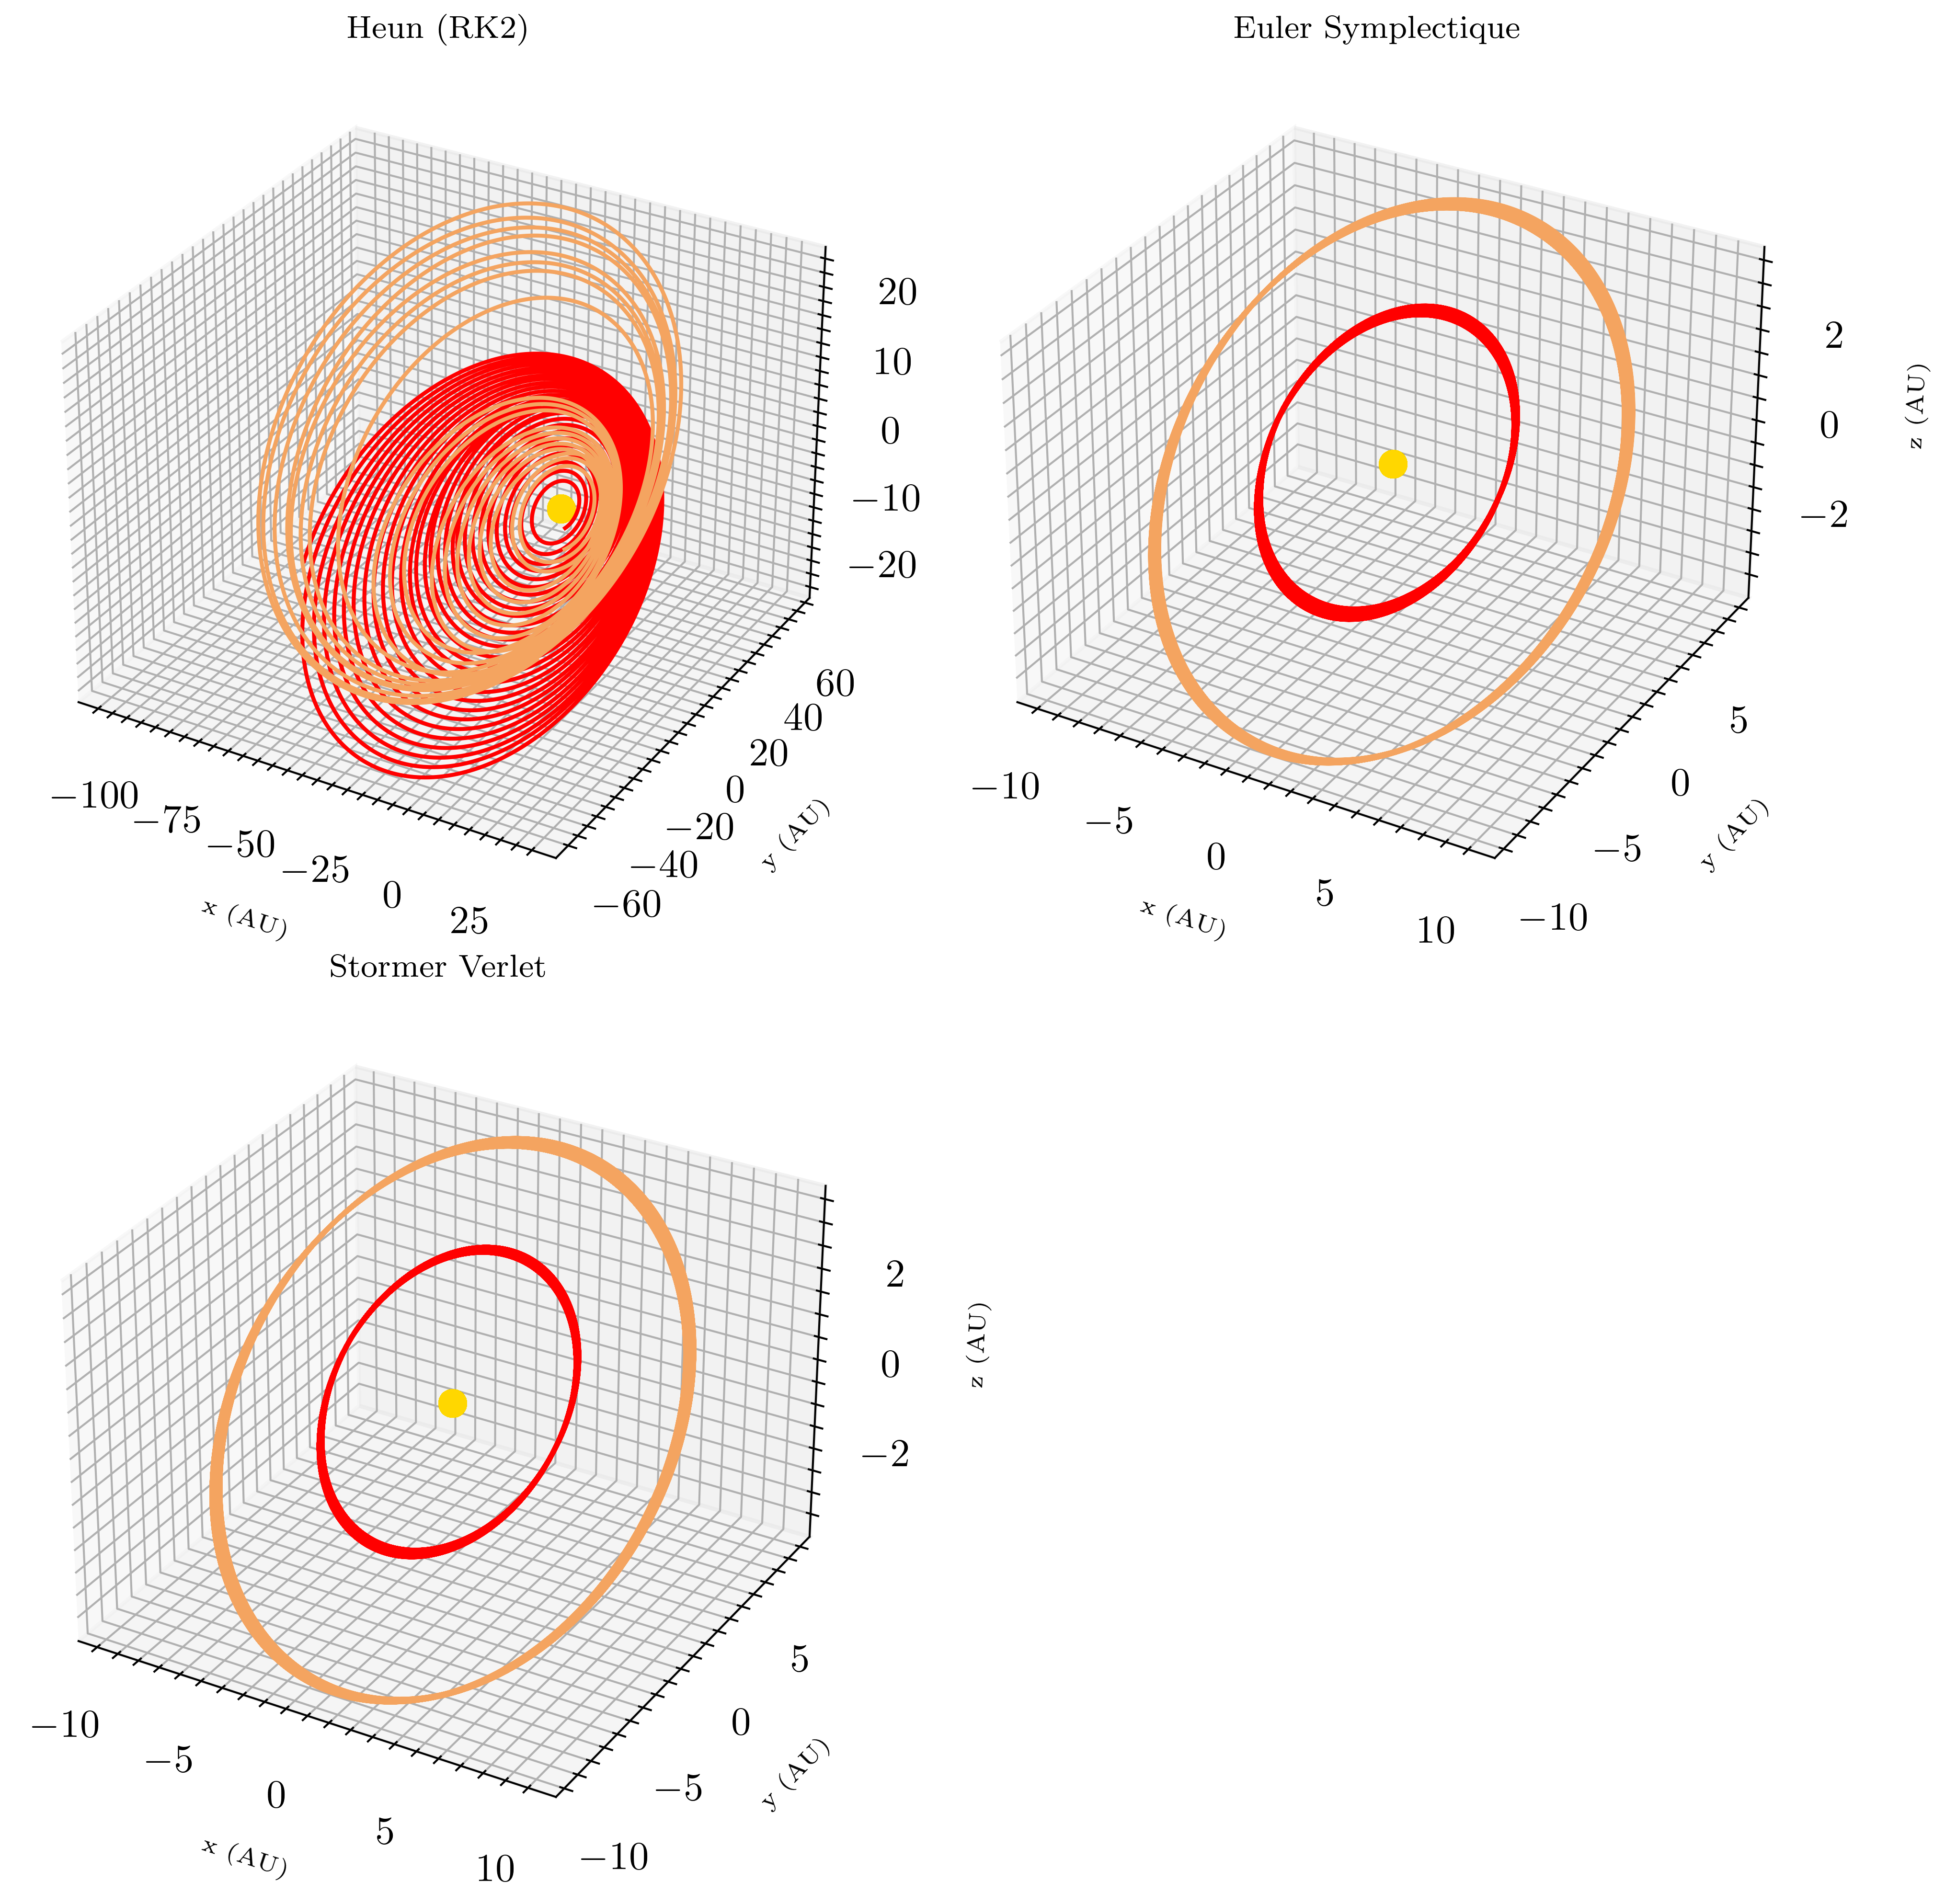
\includegraphics{figures/5000_years/orbital-plot3d.png}
  \caption{Evolution orbitale en $3$ dimension de l'orbite du Soleil (\emph{point jaune}), de Jupiter (\emph{rouge}) et de Saturne (\emph{brun}) pour les $5000$ prochaines années.}
  \label{fig:orbital-plot3D--5000}
\end{figure}

\end{document}
